\documentclass[12pt]{article}

\usepackage{lmodern}
\usepackage[T1]{fontenc}
\usepackage[spanish,activeacute]{babel}
\usepackage[utf8]{inputenc}
\usepackage{mathtools}
\usepackage{enumerate}
\usepackage{amsthm}
\usepackage{amssymb}
\usepackage{float}
\usepackage{subfig}
\usepackage{anysize}
\usepackage{wrapfig}

\marginsize{2cm}{2cm}{2cm}{2cm}

\title{Temas Ingeniería, Empresa y Sociedad}
\author{ }

\newtheoremstyle{definition_wo_parentheses}
  {\topsep}% measure of space to leave above the theorem. E.g.: 3pt
  {\topsep}% measure of space to leave below the theorem. E.g.: 3pt
  {}% name of font to use in the body of the theorem
  {0pt}% measure of space to indent
  {\bfseries}% name of head font
  {.}% punctuation between head and body
  { }% space after theorem head; " " = normal interword space
  {\thmname{#1}\thmnumber{ #2.}\thmnote{ #3}}
  
\theoremstyle{definition_wo_parentheses}	
\newtheorem{definicion}{Definición}[section]

\begin{document}
\maketitle

\section{Tema 1: La empresa y la dirección de empresas}
\textbf{Organización}: Unidad coordinada formada por un mínimo de dos personas que trabajan para alcanzar un objetivo o conjunto de objetivos comunes.\\
\textbf{Empresa}: Organizaciones que proveen bienes o servicios cuya finalidad es la obtención de beneficios (diferencia entre ingresos y gastos).\\

\subsection{Los subsistemas funcionales de la empresa}
La empresa como sistema puede ser descompuesta en subsistemas que poseen las características del sistema general. Desde una perspectiva tradicional proponemos la división de la empresa en subsistemas funcionales de: financiación, marketing, producción, investigación, desarrollo, personal, etc.\\
\textbf{Crítica}: suponer que tales subsistemas constituyen unidades aisladas, cuando en realidad están en continua interacción.\\
\textbf{Solución}: Subsistema management (administrativo).\\

\textsc{El subsistema management} tiene diferentes funciones:
\begin{enumerate}
\item \textbf{Función general}: Integrar las distintas partes y elementos de la empresa entre sí e integrar la empresa con su entorno.
\item \textbf{Funciones específicas}: 
\begin{enumerate}
\item Planificación: Implica la definición de objetivos, conductas y acciones concretas para alcanzarlos tanto a nivel global como a nivel de los diferentes subsistemas con la finalidad de proyectar la empresa en el futuro.
\item Organización: Tiene como objetivo establecer un orden interno coherente que permita a la empresa funcionar con unidad dentro y frente a su entorno. Implica la estructuración de las relaciones interpersonales y la integración y coordinación del esfuerzo de todos los miembros a pesar de intereses divergentes.
\item Dirección: Liderar, motivar y gestionar grupos.
\item Control: Debido a la naturaleza abierta del sistema empresa, es un complemento necesario para la planificación. (Controlar que todo vaya según lo previsto).
\end{enumerate}
\end{enumerate}

\textbf{Funciones gerenciales secuenciales}.\\
La \underline{planificación} (definir metas, estableces estrategias y desarrollar subplanes para coordinar las actividades), la \underline{organización} (determinar qué debe hacerse, cómo se hará y quién deberá hacerlo), la \underline{dirección} (dirigir y motivar a los participantes y resolver conflictos) y el \underline{control} (vigilar las actividades para asegurarse de que se cumplan conforme a lo planeado), en este orden, conducen a alcanzar el propósito establecido de la organización.\\

Sin embargo el proceso administrativo tiene una \textbf{naturaleza interactiva} y todas las tareas se relacionan entre sí: en \underline{planificación}, los gerentes usan la lógica y los métodos para analizar metas y acciones; en \underline{organización}, los gerentes ordenan y asignan el trabajo, la autoridad y los recursos para alcanzar las metas de la organización; en \underline{dirección}, los gerentes dirigen, influyen y motivan a los empleados para que realicen las tareas esenciales y en \underline{control}, los gerentes se aseguran de que la organización se dirige hacia los objetivos de la organización.

\section{Tema 2: El empresario}
\textbf{Empresario}: Persona o grupo de personas (órgano colegiado) que da vida a la empresa: coordina, dirige y controla el proceso productivo.

\subsection{La dirección: Funciones y niveles}
\begin{enumerate}
\item \textbf{Diferenciación vertical}: Compuesta por una alta dirección, directivos medios y supervisores de primera línea. 
\item \textbf{Diferenciación horizontal}: Compuesta por directivos generalistas arriba y directivos generalistas y directivos funcionales por debajo de los primeros directivos generalistas.
\end{enumerate}

	Como ejemplo, si una empresa tiene varias secciones para diferentes productos, pero sólo tiene un departamento, por ejemplo, de publicidad, legal o económico común a todas las secciones, será diferenciación vertical. Por el contrario, si cada sección tiene un departamento propio para estos asuntos, será diferenciación horizontal.

\begin{figure}[H]
 \centering
  \subfloat[Diferenciación Horizontal]{
   \label{f:difH}
    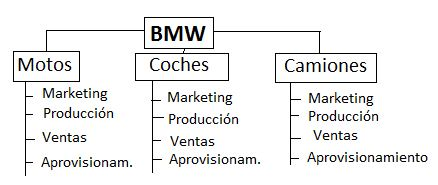
\includegraphics[width=0.5\textwidth]{difHorizontal}}
  \subfloat[Diferenciación Vertical]{
   \label{f:difV}
    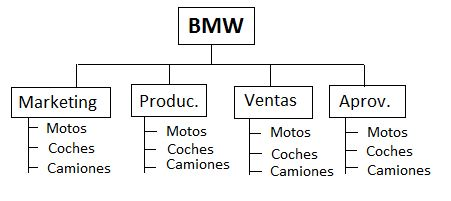
\includegraphics[width=0.5\textwidth]{difVertical}}
 \caption{Ejemplo diferenciación}
 \label{f:dif}
\end{figure}


\section{Tema 4: Organización}

\begin{definicion}[Organización] 
	Diseño del armazón material y humano que actuará de soporte para la ejecución de los planes establecidos.
\end{definicion}

\begin{itemize}
\item El punto de partida es el conocimiento de la misión, así como de los objetivos (estratégicos y operativos).

\item Utilización de diferentes herramientas (parámetros de diseños para construir la estructura. Implica tomar decisiones internas sobre: 

	\begin{itemize}
		\item Diseño de puestos de trabajo (especialización, formalización y preparación).
		\item Agrupación de puestos en unidades (departamentalización)
		\item Tamaño de las unidades.
		\item Establecimiento de vínculos laterales para coordinar departamentos.
	\end{itemize}

\end{itemize}


\subsection{Introducción a la función de organización}


\end{document}